% -----------------------------------------------
% Template for ICMC 2005
%     icmc.sty -> style file
% By Eloi Batlle (eloi@iua.upf.es), changes for 
% ICMC 2005 by Bram de Jong 
% Adapted for the ICMC 2008 by Maarten van Walstijn
% -----------------------------------------------

\documentclass{article}
\usepackage{icmc,amsmath}
\usepackage{graphicx}
\usepackage{hyperref}
\usepackage{url}
\usepackage{color}
\definecolor{black}{rgb}{0,0,0}
\hypersetup{colorlinks,urlcolor=black,linkcolor=black,citecolor=black}  
%reduces the space between the items in the itemize-environment 
\newenvironment{packed_enumerate}{
\begin{enumerate}
  \setlength{\itemsep}{1pt}
  \setlength{\parskip}{0pt}
  \setlength{\parsep}{0pt}
}{\end{enumerate}}
\newenvironment{packed_item}{
\begin{itemize}
  \setlength{\itemsep}{1pt}
  \setlength{\parskip}{0pt}
  \setlength{\parsep}{0pt}
}{\end{itemize}}

% Title.
% ------
\title{The Development of a Multidimensional Parameter Model in Max/MSP}

% Single address
% To use with only one author or several with the same address
% ---------------
% TODO: This is causing a TEX error.  Not sure why or what to do about it.  [TAP]
\oneauthor
%  {Author} {School \\ Department}
    { Timothy Place,$^{a}$ Trond Lossius,$^{b}$ Alexander Refsum Jensenius,$^{c}$ Nils Peters,$^{d}$ }
	{\affaddr{$^{a}$ Electrotap, tim@electrotap.com}\\
	\affaddr{$^{b}$ BEK - Bergen Center for Electronic Arts, lossius@bek.no}\\
	\affaddr{$^{c}$ University of Oslo, a.r.jensenius@imv.uio.no}\\
	\affaddr{$^{d}$ CIRMMT, McGill University, Montr\'eal, nils.peters@mcgill.ca} } 


% Two addresses
% --------------
%\twoauthors
%  {First author} {School \\ Department}
%  {Second author} {Company \\ Address}

% Three addresses
% --------------
%\threeauthors
%  {First author} {School \\ Department}
%  {Second author} {Company \\ Address}
%  {Third author} {Company \\ Address}

\begin{document}
%
\maketitle
%
% CHANGED: Trond commented out \sloppy as it avoided Ltypesetting in TextMate.
%\sloppy
%%%%%%%%%%%%%%%%%%%%%%%%%%%%%%%%%%%%%%%%%%%%%%%%%%%%%%%%%%%%%%%%%%%%%%%%%%%%%%%
%%%%%%%%%%%%%%%%%%%%%%%%%%%%%%%%%%%%%%%%%%%%%%%%%%%%%%%%%%%%%%%%%%%%%%%%%%%%%%%
%%%%%%%%%%%%%%%%%%%%%%%%%%%%%%%%%%%%%%%%%%%%%%%%%%%%%%%%%%%%%%%%%%%%%%%%%%%%%%%
\begin{abstract}
%The abstract should be placed at the top left column and should contain
%about 150-200 words.
The authors propose a expanded notion of how we work with parameters in computer-based environments for time-based art. Rather than viewing parameters as single points of control, the authors argue that parameters must become more multifaceted and dynamic in order to serve the needs of artists. A proposed partial solution to this problem is to give parameters additional properties that define their behavior. An example implementation of these ideas is presented in Jamoma, where these properties are themselves dynamic and interdependent upon each other.
\end{abstract}


%%%%%%%%%%%%%%%%%%%%%%%%%%%%%%%%%%%%%%%%%%%%%%%%%%%%%%%%%%%%%%%%%%%%%%%%%%%%%%%
%%%%%%%%%%%%%%%%%%%%%%%%%%%%%%%%%%%%%%%%%%%%%%%%%%%%%%%%%%%%%%%%%%%%%%%%%%%%%%%
%%%%%%%%%%%%%%%%%%%%%%%%%%%%%%%%%%%%%%%%%%%%%%%%%%%%%%%%%%%%%%%%%%%%%%%%
\section{Introduction} % (fold)
\label{sec:introduction}

Fundamental to the development of musical or artistic material is the ability to transform raw materials.  This ability implies the facility to master many facets of the material, and to manipulate it with plasticity.  Computer music environments typically provide points of control to manipulate material by providing parameters with controllable values. However, we find that this capability to control the values of parameters is inadequate for many of our artistic endeavors, and does not reflect the analogous tools and methods of artists working with physical materials. 

% Changed: Changed "audiomusical" to using the term "time-based art". See e.g. http://www.pica.org/tba/ for examples of the use of this term. [TL]
For our purposes we will assume the \emph{materials} we are working with to be media related to time-based art, such as real-time processing of audio, video, midi or other kinds of data as part of a performance. The plasticity we refer to means we want to easily shape and mold our materials into a final sonic or visual output.


\subsection{The Struggle to be Dynamic} % (fold)

Current practice for many users of computer music software is predicated on static relationships and the use of static presets. This is certainly true for many Digital Audio Workstations (DAWs) whose overall structure is fixed. It is, however, also true of open-ended systems, such as PureData or Max/MSP. In a graphical environment, the relationships between objects and their interconnections form the algorithm that determines a tool's behavior. Within this algorithm there is typically some freedom to modify its behavior by e.g. changing coefficients. However, the objects and connections generally do not change on-the-fly as a performance is executed.

Many of these systems, Max/MSP in particular, have provisions for breaking out of sets of static relationships through scripting. For the vast majority of users, however, mastering this task is onerous at best. By keeping these relationships fixed, the expressivity available to the user is inherently limited. 

To address this need for systems which are more dynamic, a possible partial solution is to treat parameters not as a single-value representing entities, but to treat parameters as a multi-dimensional tools or objects.  Thus the parameter, as a tool or object, has many facets itself in addition to the value it renders.  These many \emph{properties} of the parameter define its behavior. This paper presents a prototype of these ideas, implemented in Jamoma, a modular framework for Max/MSP \cite{Place:2006}. In addition to defining behaviors, the behaviors are themselves interdependent upon each other requiring a flexible and dynamically bound code base for the implementation.

% subsection dynamism (end)
% section introduction (end)



%%%%%%%%%%%%%%%%%%%%%%%%%%%%%%%%%%%%%%%%%%%%%%%%%%%%%%%%%%%%%%%%%%%%%%%%%%%%%%%
%%%%%%%%%%%%%%%%%%%%%%%%%%%%%%%%%%%%%%%%%%%%%%%%%%%%%%%%%%%%%%%%%%%%%%%%%%%%%%%
%%%%%%%%%%%%%%%%%%%%%%%%%%%%%%%%%%%%%%%%%%%%%%%%%%%%%%%%%%%%%%%%%%%%%%%%%%%%%%%
\section{Jamoma} %(fold)
\label{sec:jamoma}

\subsection{Model-View-Controller} %(fold)
\label{sec:mvc}

Jamoma is a Model-View-Controller (MVC) framework that provides a modular structure for the Max/MSP environment. ``MVC programming is the application of [a] three-way factoring, whereby objects of different classes take over the operations related to the application domain (the model), the display of the application's state (the view), and the user interaction with the model and the view (the controller).'' \cite{Krasner:1988}  

\subsubsection{Model / Algorithm} %(fold)
In Jamoma, the model is represented as a Max patcher or external object called the \emph{algorithm}. The algorithm is a standalone abstraction which performs the task of a module, but has no user interface and does not manage its own state.
% subsubsection (end)

\subsubsection{View / GUI} %(fold)
The user interface may consist of one or more objects in the module. These are made visible to the user by embedding the module in a bpatcher, or by opening a view of the patcher in Max. Much of the GUI is automated. Those parts which aren't are tied to the controller through various objects in the JamomaCore.
% subsubsection (end)

\subsubsection{Controller / JamomaCore} %(fold)
The controller layer is responsible for managing all of the relationships in a module, and as such plays the most important role in creating a dynamic system.  
The controller is composed of a collection of interacting and dynamically-bound objects, which we refer to as \emph{JamomaCore}. At the heart of JamomaCore is the \emph{hub}. The hub acts as a dispatcher, and it coordinates all of the activity in a module. 

The messaging model in Jamoma addresses modules using \emph{parameters} (nodes with state) and \emph{messages} (nodes which are stateless), using the Open Sound Control (OSC) protocol \cite{Wright:2003}. For the duration of this paper we will often refer only to parameters, but the concepts generally apply to both parameters and messages.

% subsubsection (end)
% subsection mvc (end)


\subsection{Dynamic Binding} %(fold)
\label{sec:dynamic_binding}

% TODO: How to cite the thing in the footnote below? [TAP]
% NOTE: I've done a lot of searching for something more 'academic' on dynamic binding, but was not able to turn up anything good. [TAP]
To implement a controller layer of the MVC framework in a way that makes it able to easily handle continuously changing relationships among the components, it is important to use a method of \emph{dynamic binding}. Dynamic binding can be used on conceptual levels, or as meaning something specific in a variety of contexts. One prevalent example of a dynamically bound environment is the Objective-C language. Objective-C documentation discusses static binding, stating that the ``constraints are limiting because they force issues to be decided from information found in the programmer’s source code, rather than from information obtained from the user as the program runs.''\footnote{\url{http://developer.apple.com/documentation/Cocoa/Conceptual/OOP_ObjC/Articles/chapter_5_section_6.html}}

Dynamic binding in Jamoma takes place on several levels.  At the highest level, a module's parameters are bound to its hub dynamically to form the Controller layer of the MVC paradigm. Then dynamic binding takes place inside of the parameters as its properties are changed.

% subsection dynamic_binding (end)

\subsection{A Multidimensional Parameter} %(fold)

The parameter is the primary interface for a user manipulating the state of a module. In most systems, the parameter has a single task: to set a variable or coefficient. While it is straightforward to understand such a simple 1-dimensional control, it does not offer the degree of nuance that, say, a sculptor has when working with clay.  

In Jamoma, the parameter is made multi-dimensional through the use of \emph{properties} and \emph{methods} in addition to maintaining the state of a value \cite{Place:2008}. A property is an aspect of the parameter which has a state. A method is simply a mechanism for doing something, such as refreshing the user interface for the parameter. These properties define the behavior for parameters by setting a value range, repetition filtering, the type of units used to express values, and how automation is applied.

Figure~\ref{fig:structure} shows a parameter in context. Within an environment, there may be many modules. Each module may have many parameters, the number of which may change dynamically. Each parameter may have many properties. These properties may address static or dynamic entities. The properties may point to a dynamic entity which itself has properties, and so on.

\begin{figure}
\centerline{\framebox{
	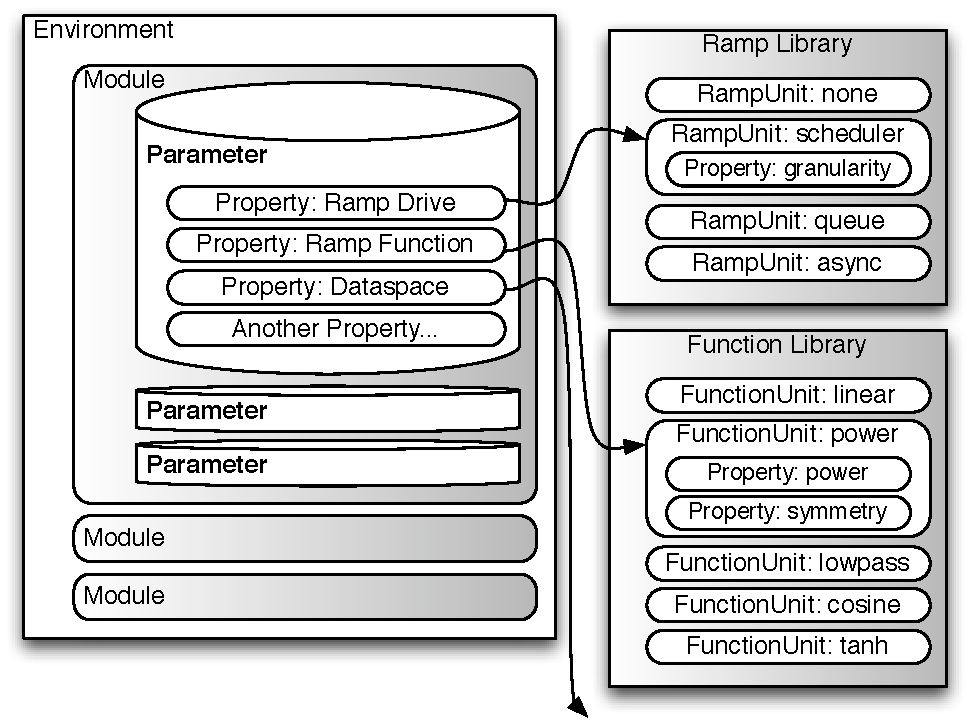
\includegraphics[width=\columnwidth]{figure-structure}}}
\caption{Parameter structure in context.}
\label{fig:structure}
\end{figure}

The example given in Figure~\ref{fig:structure} shows a number of properties. A common need is for a parameter to interpolate from its existing value to a new value.  In Jamoma we call this \emph{ramping}. Ramping is implemented in a parameter using two components: a driving mechanism and a function (shape). The driving mechanism performed by a RampUnit (discussed in Section~\ref{ssec:ramplib}) which may have properties and methods of its own. The shape of the ramp is performed by using a FunctionUnit (discussed in Section~\ref{ssec:functionlib}) which also may have properties and methods of its own. All of these are reconfigurable on-the-fly during performance.

% subsection the_parameter (end)
% section jamoma (end)


%%%%%%%%%%%%%%%%%%%%%%%%%%%%%%%%%%%%%%%%%%%%%%%%%%%%%%%%%%%%%%%%%%%%%%%%%%%%%%%
%%%%%%%%%%%%%%%%%%%%%%%%%%%%%%%%%%%%%%%%%%%%%%%%%%%%%%%%%%%%%%%%%%%%%%%%%%%%%%%
%%%%%%%%%%%%%%%%%%%%%%%%%%%%%%%%%%%%%%%%%%%%%%%%%%%%%%%%%%%%%%%%%%%%%%%%%%%%%%%
\section{Parameter Implementation} %(fold)
\label{sec:param_implementation}

At this time, the parameter object in Jamoma implements a variety of both static and dynamic properties. A parameter's behavior is ultimately determined by a compendium of these properties. %Some properties are simple values, such as the \texttt{:/repetitions} property. Other properties may be a dynamic object which itself possesses a number of properties.  Such properties include the \texttt{:/ramp/drive}, \texttt{:/ramp/function}, and various \texttt{:/dataspace} properties.
Table~\ref{tab:parameter_properties} is a brief summary of these.

%%%%%%%%%%%%%%%%%%%%%%
% CHANGED: There isn't room for this kind of detail...
%\subsection{Controlling the User Interface} % (fold)
%\label{sub:controlling_the_user_interface}
%
%In certain applications the CPU overhead of continuously updating the graphical user interface whenever parameter or message values change might become a burden, competing for CPU with e.g. video processing algorithms. If the user does not need continuous visual feedback on updated values of parameters or messages, the GUI for the parameter or message can be frozen, freeing up the processor and GPU for tasks considered more important:
%
%\texttt{:/ui/freeze}
%
%\texttt{:/ui/freeze/get}
%
%A parameter or message that has its GUI frozen can be forced to update and refresh the displayed value once by means of the message:
%
%\texttt{:/ui/refresh}

% subsection controlling_the_user_interface (end)

The parameter is implemented as a Max external called \emph{jcom.parameter}. Within jcom.parameter, the ramp and dataspace properties are implemented internally as dynamically bound objects located in a set of shared libraries.  These shared libraries are called the FunctionLib, RampLib, and DataspaceLib respectively.


\begin{table}
\begin{center}
\footnotesize\noindent
\begin{tabular}{| l | p{4.5cm} |}
    \hline
    \textbf{Property}          & \textbf{Description}\\ 
	\hline
	\texttt{:/value}			& Value of the parameter \\
	\hline
	\texttt{:/value/stepsize}	& Size of step taken \texttt{inc} and \texttt{dec} \\
	\hline
	\texttt{:/value/inc}		& Increase the value \\
	\hline
	\texttt{:/value/dec}		& Decrease the value \\
	\hline
	\texttt{:/value/default}	& Initial value \\
	\hline
	\texttt{:/type} 			& Type of data \\
	\hline
	\texttt{:/priority} 		& Order for recalling values from a preset \\
	\hline
	\texttt{:/ui/freeze} 		& Stops GUI updates to save CPU \\
	\hline
	\texttt{:/ui/refresh} 		& Updates the GUI \\
	\hline
	\texttt{:/ramp/drive} 		& Timing mechanism for ramps \\
	\hline
	\texttt{:/ramp/function} 	& Interpolation shape for ramps \\
	\hline
	\texttt{:/repetitions} 		& Filter out repeated values \\
	\hline
	\texttt{:/range/bounds} 	& Set a low and high range \\
	\hline
	\texttt{:/range/clip} 		& What to do when the range is exceeded \\
	\hline
	\texttt{:/description} 		& Documentation \\
	\hline
	\texttt{:/node/type} 		& ``parameter'' or ``message'' \\
	\hline
	\texttt{:/node/name} 		& Parameter's name \\
	\hline
	%\texttt{:/dataspace} 		& Class of values being controlled. \\
	%\hline
	%\texttt{:/dataspace/unit/active} 	& The measurement unit used when values are sent \\
	%\hline
	%\texttt{:/dataspace/unit/native} 	& The measurement unit used by the internal algorithm \\
	%\hline
\end{tabular}
\end{center}
\caption{Parameter properties in Jamoma}
\label{tab:parameter_properties}
\end{table}



%%%%%%%%%%%%%%%%%%%%%%%%%%%%%%%%%%%%%%%%%%%%%%%%%%%%%%%%%%%%%%%%%%%%%%%%%%%%%%%
%%%%%%%%%%%%%%%%%%%%%%%%%%%%%%%%%%%%%%%%%%%%%%%%%%%%%%%%%%%%%%%%%%%%%%%%%%%%%%%
%%%%%%%%%%%%%%%%%%%%%%%%%%%%%%%%%%%%%%%%%%%%%%%%%%%%%%%%%%%%%%%%%%%%%%%%%%%%%%%
\section{The Jamoma Libraries} % (fold)
\label{sec:the_jamoma_libraries}

% CHANGED: Trond is trying a different approach to this material, giving a more intuitive introduction to it, or not...

Presets and automation can be considered archetypes of strategies for dynamic controll of material. Presets in their purest form is a vertical-only approach; all values are instantly set to a certain state. On the other hand automation in its purest form is a horizontal-only approach; a fixed stream of timetagged values progressing over a limited amount of time to control the state of one parameter, often with interpolation from one value to the next. While presets are widely used in real-time signal processing environments, the use of automation is fundamental to linear time-based media software such as digital audio workstations and video editing software.

One obvious way of expanding the flexibility of presets is by implementing a cross-fade or gradual transition to the new preset by means of interpolation. Several works have expanded this further by presenting the set of presets as points in a dataspace and develop strategies of traversing that dataspace, creating dynamic interpolations between two or more presets \cite{Momeni:2003, Bencina:2005metasurface}. The former has been extensively used by one of the authors for developing the Hipno audio plugins \cite{Place:2005hipno}.

Recent development of Jamoma has aimed at expanding the possibilities for complex transitions of parameters in time. While Jamoma previously offered possibilities of ramping to a new value over a certain amount of time by means of linear interpolation, this has recently been expanded by reimplementing ramping as a combination of two libraries. 




%%%%%%%%%%%%%%%%%%%%%%%%%%%%%%%%%%%%%%%%%%%%%%%%%%%%%%%%%%%%%%%%%%%%%%%%%%%%%%%
%%%%%%%%%%%%%%%%%%%%%%%%%%%%%%%%%%%%%%%%%%%%%%%%%%%%%%%%%%%%%%%%%%%%%%%%%%%%%%%
%%%%%%%%%%%%%%%%%%%%%%%%%%%%%%%%%%%%%%%%%%%%%%%%%%%%%%%%%%%%%%%%%%%%%%%%%%%%%%%
\subsection{The Ramp Library} % (fold)
\label{ssec:ramplib}

% TODO: gear this more towards artistic, and less toward technical implementation. Try to explain the motivation for the design decisions we've made.

Depending on the circumstance it might be desirable to generate new interpolated values in different ways during the ramp: Several real-time signal processing environments distinguish between audio rate and control rate signals. Depending on the transients of the ramping signal it might sometimes be desireable to perform interpolation at audio rate, at other time it might be sufficient to update at  control rate. If the parameter is controlling a video processing algorithm it might be sufficient to update the value once per video frame processed.

% Jamoma offers vastly extended possibilities in how ramping can be done as compared to Max. In Jamoma the process of ramping is made up from the combination of two components: A driving mechanism cause calculations of new values at desired intervals during the ramp, while a set of functions offers a set of curves for the ramping. Both components are implemented as C++ APIs, and can easily be extended with new ramp or function \emph{units}, expanding the range of possible ramping modes. %TODO: Is this important for the ICMC audience that the Ramplib API is made with C++ and that it be can easily extended? [NP]

% TODO: Tim notes that the 'c++ API' and maybe other parts are common to all of the libs, and so maybe should go in the section rather than this subsection. Trond thinks that I'd like to start out with a more descriptive approach, focusing on the use of it, before delving into the technical issues. I just mention the c++ in passing.


The Jamoma RampLib, implemented as a C++ API, provides a means by which to create and use \emph{ramp units} in Jamoma.  A ramp unit is a self-contained algorithm that can slide from an existing value to a new value over a specified amount of time according to different timing mechanisms. Currently four such ramp units are implemented:

\begin{itemize}
	\item \emph{none} - jumps immediately to the new value. Typically used for values where ramping do not make sense.
	\item \emph{scheduler} - use the Max internal clock to generate new values at fixed time intervals.
	\item \emph{queue} - ramping using the Max queue, updating values whenever the processor has free capacity to do so.
	\item \emph{async} - only calculate new values when requested to do so. This might be used in video processing modules to calculate fresh values immediately before processing the next video image or matrix.
\end{itemize}

The RampLib can easily be extended with more ramp units, and one planned extension is the implementation of audio rate ramping.

When a new ramp is started, the ramp unit internally use a normalized ramping value, increasing linearly from $0.0$ to $1.0$ over the duration of the ramp. Whenever the ramp unit is to provide a new value, it updates the normalized ramping value, and pass it to a Function Unit as described in Section~\ref{ssec:functionlib}. The normalized value returned is then scaled to the range defined by the start and end values for the ramp, and passed on to the module.


% subsection ramplib (end)

%%%%%%%%%%%%%%%%%%%%%%%%%%%%%%%%%%%%%%%%%%%%%%%%%%%%%%%%%%%%%%%%%%%%%%%%%%%%%%%
\subsection{The Function Library} % (fold)
\label{ssec:functionlib}

The Jamoma FunctionLib API provides normalized mappings of values $x \in [0,1]$ to $y \in [0,1]$ according to functions $y = f(x)$. Currently five functions are implemented: 

\begin{itemize}
	\item Linear: $y = x$.
	\item Cosine: $y = - \frac{1}{2} \cdot cos(x \cdot \pi ) + \frac{1}{2} $.
	\item Lowpass series: $y[n] = y[n-1] \cdot k + x[n] \cdot (1-k)$, \\ where $k$ is a feedback coefficient.
	\item Power function: $ y = x^{k} $, parameter $k$ can be set.
	\item Hyperbolic tangent: $ y = c \cdot (\tanh(a\cdot(x-b)) - d) $, \\ where coefficients $a$, $b$, $c$, $d$ depends on the width and offset of the curve.
\end{itemize}

The FunctionLib can easily be expanded by introducing new functions as C++ files. There are immediate plans for introducing additional exponential functions.
 
% TODO: Would it be useful with a figure here?





% TODO: I don't understand the purpose of this table, and suggest we get rid of it. - TL

\begin{table}
\begin{center}
\footnotesize\noindent
\begin{tabular}{|l|l|l|l|l|l|}
\hline
          & Cosine & Linear & Lowpass & Power & Tanh \\
\hline
Scheduler &        &   x    &         &       & \\
\hline
Queue	  &        &        &         &       & \\
\hline
None	  &        &        &         &       & \\
\hline
Async	  &        &        &         &       & \\
\hline
\end{tabular}
\end{center}
\caption{The possible ramping configurations in Jamoma}
\label{tab:ramp_possibilities} %FIXME: this table has no reference to the text
\end{table}




The Jamoma libraries deliver a shared resource to all of the Jamoma framework for applying mathematical functions, converting units, and ramping. For example, the ramping functionality is not only implemented in parameters, but also in messages, special ramping objects, and in other places. The tools implemented in the libraries are pervasive throughout the environment.

Each of the libraries furnish a clear programming interface so that they are easily extendable. The dynamic binding implementation in the Jamoma framework means that by simply creating one \emph{unit} (object), it is immediately available to the rest of the Jamoma environment with no additional upkeep or maintenance elsewhere in the code.

The libraries can also be queried to find out what functionalities exist. This happens at several levels.  For example, a user may wish to find out what functions exist for doing a mathematical mapping. The FunctionLib can provide a list of available FunctionUnits. Having chosen a FunctionUnit, the user can then query to find out what additional properties (if any) the FunctionUnit has published for access. A good user interface will automate all of this querying to simply provide updated selections and options.

Currently there are three libraries in the Jamoma framework:
\begin{itemize}
	\item FunctionLib: a library of FunctionUnits which map an input value to an output value
	\item RampLib: a library of driving mechanisms (RampUnits) which use the FunctionLib to automate value transformations over time.
	\item DataspaceLib: a library by which a parameter or message can be given a class that describes the type of data it represents.  Values may then be set by any of a number of DataspaceUnits to allow control of a parameter in any of a number of ways.
\end{itemize}






% section functionlib (end)

\subsection{Interdependencies}\label{sec:interdependencies}

One of the largest potentials of the system we have outlined is that these dynamically bound libraries can be used together. One simple example of this is how a ramp drive mechanism can be paired with a function that determines the ramp's shape, and a dataspace determining what kind of unit to use for ramping.  This provides for many possibilities.
% TODO: should we just stick the above statement into the Discussion and cut this subsection? [TAP]


% section the_jamoma_libraries (end)


%%%%%%%%%%%%%%%%%%%%%%%%%%%%%%%%%%%%%%%%%%%%%%%%%%%%%%%%%%%%%%%%%%%%%%%%%%%%%%%
%%%%%%%%%%%%%%%%%%%%%%%%%%%%%%%%%%%%%%%%%%%%%%%%%%%%%%%%%%%%%%%%%%%%%%%%%%%%%%%
%%%%%%%%%%%%%%%%%%%%%%%%%%%%%%%%%%%%%%%%%%%%%%%%%%%%%%%%%%%%%%%%%%%%%%%%%%%%%%%
\section{Discussion and further work} % (fold)
\label{sec:discussion_and_further_work}

The problem: 
It has been too static
    - too difficult to create dynamic setups
    - for example, dynamic setups in Max using scripting: ick!

Trying to create something that is more flexible, but also easier to work with at the same time.

Splitting up and identify the way we handle structures in Max and put them together.  It has been very static and preset-based.

As we've been working on this for along, we hit a wall and needed to move forward, and did so by creating these libs to extend Max.  

No one wants to have to manually do all of the house-keeping to get this functionality, so we've made it largely encapsulated behind the scenes.


\cite{Momeni:2003}



4 ramp units times 5 function units = 20 ramping modes

ramp units can be used for other scheduled processes as well

Possibility of expanding ramp units as low frequency oscillators

function units can be used elsewhere, e.g. for mapping

Audio rate ramp unit.



Querying - we propose a different system to the Lemur OSC2 draft

Ramp Lib and Function Lib can be used outside the context of jcom.parameter and jcom.value: jcom.map and jcom.ramp


Plans to extend the FunctionLib by introducing exponential functions are under discussion. %CHANGED: move this from the FunctionLib to Future Work [NP] 


* ramping with our own scheduler to take the burden off of the Max scheduler.


\subsection{DataspaceLib} %(fold)
\label{sec:dataspacelib}

When sending values to a parameter, it is important to know what kind of value the parameter expects.

Depending on the circumstance it might be desirable to generate new interpolated values in different ways during the ramp: Several real-time signal processing environments distinguish between audio rate and control rate signals. Depending on the transients of the ramping signal it might sometimes be desireable to perform interpolation at audio rate, at other time it might be sufficient to update at  control rate. If the parameter is controlling a video processing algorithm it might be sufficient to update the value once per video frame processed.

%The DataspaceLib is important because...
%using different unit types and moving toward more perceptual/semantic representations instead of being chained to technical terms.
%
%It will be good for us to try and explain all the interactions here ;-) 
%\begin{packed_item}
%	\item AngleDataspace
%	\item NoneDataspace
%	\item ColorDataspace
%	\item PitchDataspace
%	\item PositionDataspace
%	\item DistanceDataspace
%   \item TemperatureDataspace
%    \item GainDataspace
%	\item TimeDataspace
%\end{packed_item}
%	
%%%%%%%%%%%%%%%%%%%%%%%%%%%%%%%%%%%%%%%%%%%%%%%%%%%%%%%%%%%%%%%%%%%%%%%%%%%%%%%
%\subsubsection{TemperatureDataspace}\label{subsec:temperature_dataspace}
%
%La de da...right now 1ºC in Montreal %TODO: not necessary, or should go to the Dataspace subsection [NP]


% subsection dataspacelib (end)


% section discussion_and_further_work (end)


%\begin{thebibliography}{citations}
%
%\bibitem{Author:00} Author, E.
%''The title of the conference paper'',
%{\it Proceedings of the International Computer Music Conference}, Miami, USA, 2004.
%
%\bibitem{Someone:02} Someone, A.
%{\it  Title of the book}.
%Publisher, Belfast, 2007.
%
%\end{thebibliography}

% Bibliography (fold)
%
% The following two commands are all you need in the initial runs of your .tex file to
% produce the bibliography for the citations in your paper.
% CHANGED: I remove the small again for the bibliography, since this isn't used in the template.
%\begin{small}
\bibliographystyle{abbrv}
\bibliography{jamoma-icmc2008}  % the name of the Bibliography in this case
%\end{small}
% You must have a proper ".bib" file
%  and remember to run:
% latex bibtex latex latex
% to resolve all references
%
% Bibliography (end)



\end{document}
